% file: reasoning_case.tex

\begin{ReasoningBox}[title=Etiological Reasoning] % 可以通过 title 参数修改标题
    % --- 第一部分：问题描述与图片 ---
    % \begin{minipage}[t]{0.58\textwidth}
    \begin{wrapfigure}{r}{0.3\textwidth}
        \centering
        % wrapfigure 通常顶部会有多余空白，使用负 vspace 向上提，让图片和第一行文字对齐
        \vspace{-20pt} 
        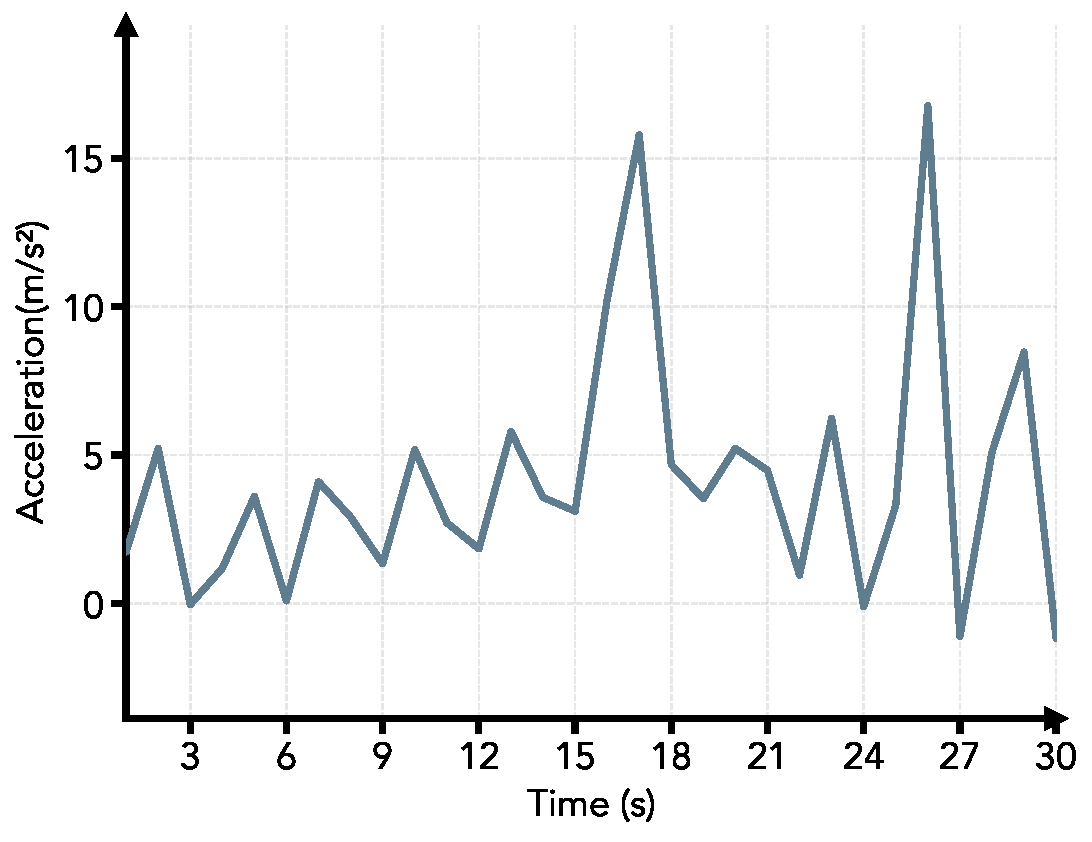
\includegraphics[width=\linewidth]{blocks/sample_cases_success/etiological.pdf}
        % 调整底部的留白
        \vspace{-20pt}
    \end{wrapfigure}
        \textbf{Question:} You are given a short tri-axial accelerometer time series collected at a sampling rate of 20~Hz from a subject performing a physical activity. The sequence consists of 10 consecutive timestamps (approximately 0.5 seconds), where each timestamp contains acceleration measurements along the X, Y, and Z axes, yielding a total of 30 values formatted as:
\[
[x_1, y_1, z_1, x_2, y_2, z_2, \dots, x_{10}, y_{10}, z_{10}].
\]

Acceleration values lie in the range $[-20, 20]$, where 10 corresponds to $1g$ (approximately $9.8~\text{m/s}^2$), and the measurements include gravitational acceleration. Consequently, when the device is stationary on a flat surface, the vertical axis typically registers approximately $\pm10$. The subject is performing one of the following six activities:
\textit{walking}, \textit{jogging}, \textit{sitting}, \textit{standing}, \textit{upstairs}, or \textit{downstairs}. Given the provided accelerometer time series, identify the activity label that most likely generated the data.

    \vspace{0.5em}

    % --- 第二部分：选项 ---
    \textbf{Answer Choices:} \\ (A) Walking \\ (B) Jogging \\ (C) Upstairs \\ (D) Downstairs \\ (E) Sitting \\ (F) Standing \\
    \textbf{Correct Answer:} \textcolor{correctgreen}{(D)} \\
\end{ReasoningBox}